\onehalfspacing

\section{Capisaldi di Design}
Sono stati fissati \textit{\textbf{tre punti chiave}} che devono essere rispettati durante l'implementazione del firewall virtuale \cite{bakker2016network}:
\begin{itemize}
  \item Un firewall basato su OpenFlow deve essere in grado di \textit{\textbf{filtrare il traffico in modo simile ad un firewall tradizionale}}, tramite la definizione di regole di flusso.
  \item Dovrebbe essere possibile \textit{\textbf{distribuire le regole su un'intera rete senza la necessità di configurare gli switch uno alla volta}}; ciò affronta il problema di proteggere un'intera infrastruttura di rete da minacce sia interne che esterne.
  \item Poiché non si può presumere che le reti siano omogenee, dovrebbero essere implementate \textit{\textbf{su una rete politiche di sicurezza eterogenee}}; ciò richiede l'implementazione di un meccanismo che consente a diverse parti di una rete di filtrare diversi flussi di traffico (vedasi nei paragrafi successivi).
\end{itemize}

\section{Componenti principali}

Per poter implementre le proposte citate nella sezione \ref{firewall_confini}, è stato sviluppato \code{ACLSwitch}\footnote{\url{https://github.com/bakkerjarr/ACLSwitch}}, un'applicazione sviluppata tramite il controller \textit{framework Ryu} che si propone come firewall virtuale distribuito su tutta una determinata rete.

Altri componenti importanti sono le \textit{\textbf{Access Control List}} (ACL) e le \textit{\textbf{Policy Domains}} (Politiche di Dominio). L'implementazione effettuata ad-hoc delle ACL eredita tutti i concetti dei firewall tradizionali; mentre l'inclusione delle Politiche di Dominio \textit{estende} le attuali capacità degli attuali Firewall basati su OpenFlow, fornendo all'amministratore di rete meccanismi di distribuzioni delle regole ACL a gruppi di switch senza la necessità di configurare in maniera separata ognuno di essi. Il metodo di creare regole singole poi distribuirle a dispositivi specifici è tipico sia dei firewall tradizionali che di basati su OpenFlow. Tramite \textit{ACLSwitch} questa funzionalità viene aumentata presentando un meccanismo per raggruppare le regole in \textit{policy domains} che nel pragrafo seguente verranno meglio esplicate.

\section{ACL Estese}

Le capacità delle ACL sono state estese aggiungendo campi extra oltre alle solite 5 tuple (vedasi \ref{firewall_cont}) risultando come segue \cite{bakker2016network}:

\[
  \text{regola ACL } r = \overbrace{
    ip\_src, ip\_dst, tp\_proto, port\_src, port\_dst
   }^\text{Le 5 tuple ACL base},
   \overbrace{
    policy, action, time\_start, time\_duration
   }^\text{Estensioni}
 \]

I nuovi campi si identificano come segue:
\begin{itemize}
  \item \textbf{\textit{policy}}: è il primo campo ed identifica la politica di dominio di cui fa parte la regola.
  \item \textbf{\textit{action}}: indica, come suggerisce il nome, l'azione da intraprendere, per esempio se un certo traffico che matcha debba essere inoltrato o scartato.
  \item \textbf{\textit{time\_start}} e \textbf{\textit{time\_duration}}: sono campi facoltativi ed indicano rispettivamente la data di inizio e la durata in cui la regola debba essere in vigore.
\end{itemize}

\subsection{Policy Domains}

Un policy domain rappresenta una relazione tra le regole ACL e gli switch OpenFlow. Un policy domain può contenere molte regole ACL ma ogni singola regola ACL può essere membro di un solo policy domain. Un policy domain può essere assegnato a molti switch e ad ogni switch possono essere assegnati più policy domain (Fig. \ref{fig:domains}).

L'astrazione fornita dai policy domain consente a un'intera rete di essere protetta da una singola politica e, per estensione, da un singolo meccanismo. Tuttavia, offrono anche la flessibilità di assegnare diversi gruppi di regole a switch separati e, per estensione, a punti diverse della stessa rete.

\begin{figure}[H]
  \centering
  \begin{subfigure}[b]{0.46\linewidth}
    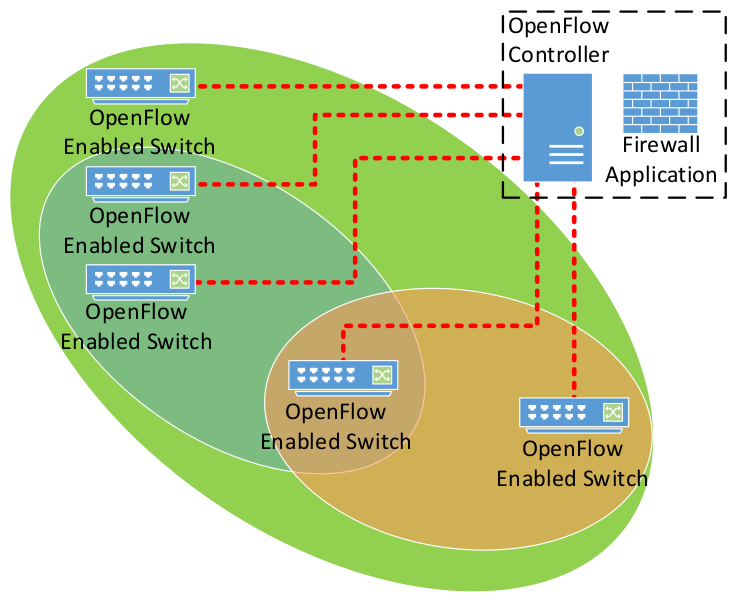
\includegraphics[width=\linewidth]{img/domains.png}
    \caption{I policy domains (ellissi colorate) possono essere assegnati a switch per proteggere simultaneamente l'intera rete e mettere in vigore altre politiche \cite{bakker2016network}}
    \label{fig:domains}
  \end{subfigure}
  \begin{subfigure}[b]{0.46\linewidth}
    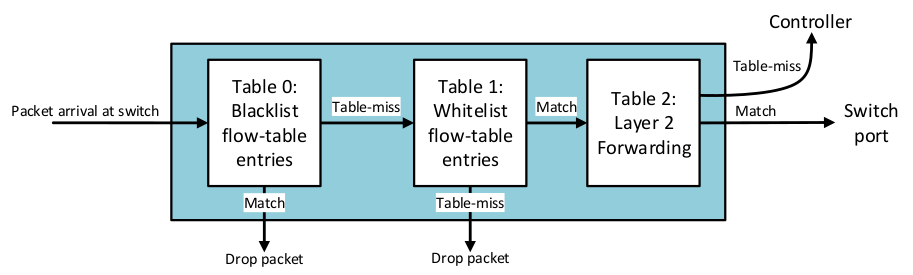
\includegraphics[width=\linewidth]{img/pipeline.png}
    \caption{Implementazione della pipeline \cite{bakker2016network}}
    \label{fig:pipeline}
  \end{subfigure}
\end{figure}

\section{Deploy delle Flow Table Entries}

OpenFlow supporta due stili di distribuzione delle FTE: \textit{deploy reattivo} e \textit{deploy proattivo}.

Il \textbf{\textit{deploy reattivo}} viene utilizzato dal controller come risposta a un messaggio \code{packet-in} da uno switch. Quando si creano firewall utilizzando OpenFlow, questa modalità non è adatta a causa del non trascurabile overhead che impone al controller per elaborare decisioni sul traffico.

Questo problema viene risolto \textit{deployando in modalità proattiva} agli switch le FTE nel momento in cui vengono create le regole ACL.

\section{Pipeline}\label{pipeline}

Come mostrato in Fig. \ref{fig:pipeline}, la pipeline è la seguente \cite{bakker2016network}:
\begin{itemize}
  \item \code{Table 0} è la prima tabella della pipeline e contiene FTE associate a bloccare flussi di traffico facenti parte di una lista nera; in altre parole i pacchetti che matchano vengono scartati. I pacchetti che corrispondono alla voce \code{table-miss} vengono inoltrati alla \code{Table 1} tramite l'azione \code{Goto-Table}. Pertanto, questa tabella viene utilizzata per fare una prima scrematura, bloccando flussi di traffico \textbf{\textit{indesiderati}}.

  \item \code{Table 1} è la tabella successiva nella pipeline, contiene FTE associate a far passare flussi di traffico facenti parte di una lista bianca; in altre parole i pacchetti che matchano vengono direttamente inoltrati alla \code{Table 2}, il resto, ossia quelli che corrispondono alla \code{Table-miss} vengono scartati.

  \item \code{Table 2} esegue il ruolo di un normale switch ethernet.
\end{itemize}
